\begin{figure}[h!]
    \centering
    \caption{Probability of being a renter by (residualized) household income decile}
    \label{fig:ahs_pr_renters}

    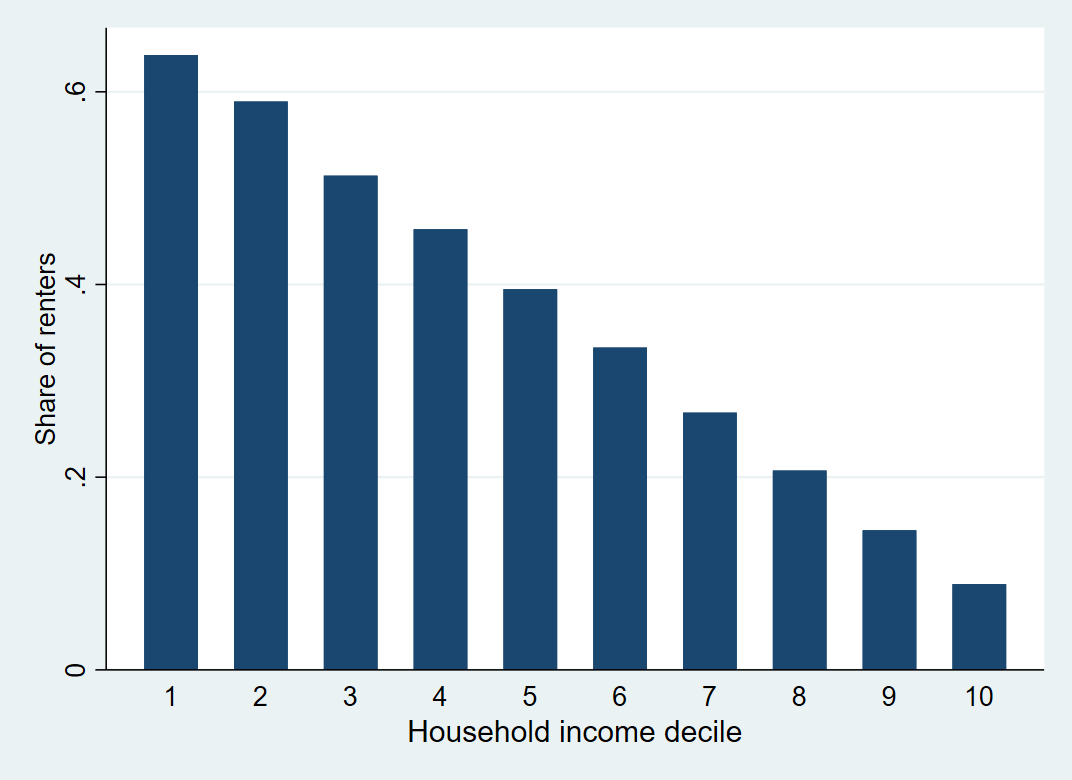
\includegraphics[width = 0.75\textwidth]{ahs/output/sh_renters.png}

    \begin{minipage}{.95\textwidth} \footnotesize
        \vspace{3mm}
        Notes: Data are from the 2011 and 2013 American Housing 
        Survey (AHS), as described in Section \ref{ADD SECTION}. 
        The figure shows the distribution of the probability of 
        renting by household income. 
        Both the probability of being a renter and the household income
        are residualized at the SMSA level.
        We exclude from the calculation non-conventional housing units, 
        such as mobile homes, hotels, rooming houses, etc.
    \end{minipage}
\end{figure}
